%% This document gives an example on how to use the ntnubachelorthesis
%% LaTeX document class.
%% Use oneside for PDF delivery and twoside for printing in a book style
%% use language english, norsk, nynorsk and one of the following shortenings
%%  ``BSP'' Bachelor i Spillprogrammering,\\
%%  ``BRD'' Bachelor i drift av nettverk og datasystemer,\\
%%  ``BIS'' Bachelor i Informasjonssikkerhet,\\
%%  ``BPU'' Bachelor i Programvareutvikling, \\
%%  ``BIND'' Bachelor i Ingeniorfad - data, \\
%%  ``BADR'' Bachelor i drift av datasystemer, \\
%%  ``BIT'' Bachelor i informatikk, \\
%%  ``BABED'' Bachelor i IT-støttet bedriftsutvikling.
%%   for example \documentclass[BIS,norsk,twoside]{ntnuthesis/ntnubachelorthesis}

\documentclass[BIND,norsk,oneside]{ntnuthesis/ntnubachelorthesis}

\usepackage{csvsimple}
\usepackage{booktabs}

\usepackage{gnuplottex}


\definecolor{darkgreen}{rgb}{0,0.5,0}
\definecolor{darkred}{rgb}{0.5,0.0,0}

\lstset{        basicstyle=\ttfamily,
                keywordstyle=\color{blue}\ttfamily,
                stringstyle=\color{darkred}\ttfamily,
                commentstyle=\color{darkgreen}\ttfamily,
}


%Typesetting of C++
\newcommand{\CPP}[0]{{C\nolinebreak[4]\hspace{-.1em}\raisebox{.1ex}{\small\bf +\hspace{-.1em}+\ }}}



%\newcommand{\comment}[1]{\textcolor{blue}{\emph{#1}}}  %% use of the colour and you can see how to use commands with parts \comment{so what}

%% The class files defines these two
%% \newcommand{\NTNU}{Norwegian University for Science and Technology} %

% you can create you one #define like structures using the \newcommand feature
% you can change behaviour using \renewcommand

\newcommand{\com}[1]{{\color{red}#1}} % supervisor comment
%\renewcommand{\com}[1]{} %remove starting % to remove supervisor comments
% This will appear in text \com{Lecuters comment} and be visible unless you uncomment
% the renewcommand line.

\newcommand{\todo}[1]{{\color{green}#1}} % items to do
%\renewcommand{\todo}[1]{} %remove starting % to remove items to do

\newcommand{\n}[1]{{\color{blue}#1}} % other comment
%\renewcommand{\n}[1]{} %remove starting % to remove notes

\newcommand{\dn}[1]{} % add the d to a note to say that you have finished with it.

\newcommand{\gj}{NTNU i Gj\o{}vik}


% Norwegian Characters,  needs the {} or to be separate from the next letters
% \o{}   \aa{}   \ae{}   so at the end of a word you can use \o  \aa   \ae
% \O{}   \AA{}   \AE{}   you can also just leave a space and latex will remove it
%    eg, NTNU i Gj\o vik  or NTNU i Gj\o{}vik





\begin{document}

\thesistitle{Example Game Programming Thesis. With a long title to test the wrapping of the box}
\thesisshorttitle{Example Game Programming Thesis} % use this if you have a very long title and want something shorter on the header pages
\thesisauthor{Simon McCallum}
\thesisauthorA{Ivar Farup}
%\thesisauthorB{}
%\thesisauthorC{}
\thesissupervisor{Rune Hjelsvold}
%\thesissupervisorA{john smith} %second supervisor

%\thesisOppgaveNo{29E}

\nmtkeywords{Thesis, Latex, Template, IMT}
\nmtdesc{This is the short description of a bachelor thesis. It should contain a short introduction to the area of the thesis and what the thesis contributes to that area. This does not allow for paragraphs so you have to include the entire short description in a single paragraph.}

\nmtoppdragsgiver{\NTNU}
\nmtcontact{Erik Helm\aa s, erik.helmas@ntnu.no, 61135000}




\thesisdate{\ntnubachelorthesisdate}
\useyear{18.05.2016}

\nmtappnumber{} %numebr of appendixes
\nmtpagecount{} %currently auto calculated but might be wrong




\thesistitleNOR{Norwegian title.}
\nmtkeywordsNOR{Norway, Norsk}
\nmtdescNOR{Dette b\o{}r være p\aa norsk, jeg tenkte jeg skulle legge til litt mer tekst 
\aa s\o{}rge for at det gikk over flere linjer. Jeg m\aa sjekke p\aa siden 
nummer Feild som det kanskje burde være kun de sidene uten 
vedlegg. Forel\o{}pig returnerer den siste siden av hele dokumentet. 
Hvis jeg ikke kan finne ut av det, vil jeg gi to innganger, gmtnumberpages og gmtappnumber. 
Det burde gj\o{}re jobben. (done in google translate so it is bad norwegian) }

 % this is the file which contains all the details about your thesis

\makefrontpages % make the frontpages

\input{inc/preface}


\tableofcontents
\listoffigures
\listoftables
\lstlistoflistings


\input{inc/introduction}
\chapter{Requirements}
\label{chap:requirements}

The title of the thesis should be set using the \verb+\thesistitle+
command, and the date of the thesis should be set using the
\verb+\thesisdate+ command. This makes the title and date appear in
the running header, like in this document.

\section{Page Layout}

The geometry of the page has been set using the \verb+\geometry+
command. 

\section{Fonts}

Due to limited \LaTeX\ support for the Georgia font, Charter has been
chosen instead. For mathematical formula, the Euler fonts are used,
since they blend more nicely with the Charter than the standard
\LaTeX\ fonts: 
$$
 f(x) = \int_0^x g(\tau)\,d\tau
$$

For inline math you can use $\backslash{}($ and $\backslash{})$ for example \( f(x)= \frac{x^2}{1+x^2} \).  
This also allows you to use $\slash$ and $\backslash$. You need to include the \{\} when you want the special
character to have other letters immediately after it.

\section{Sectioning Commands}

The standard \LaTeX\ sectioning commands are used for both numbered
and unnumbered sections. The top level is given by the \verb+\chapter+
command. This starts a new right page. The two lower levels are
obtained using the \verb+\section+ and \verb+\subsection+ commands.
The standard \LaTeX\ \verb+\subsubsection+ and \verb+\paragraph+
commands have been disabled since their use is not encouraged by the
thesis guidelines. When you use these they will not be given numbers.  
They still appear in the document with highlighting but not in the 
table of contents.

\subsection{The subsection}

This is an example of a subsection.

\subsubsection{The subsubsection}

This is an example of a subsubsection.

\paragraph{The paragraph}

This is an example of a paragraph with a heading.

\section{Floats (Figures and Tables)}
\label{sec:floats}

Figures are placed in the \texttt{figure} environment. An example is
shown in Figure~\ref{fig:examplegnuplot}. %notice the ~ in between figure and the \ref. it stops latex from splitting the number and word over a line.
You can make nicer graphs using gnuplot, for example see Figure~\ref{fig:examplegnuplot}.

Tables are placed in the \texttt{table} environment. An example is given in
Table~\ref{tab:example1}. Figures and tables float freely around in the
document in accordance with standard \LaTeX\ behavior.

\begin{figure}[htbp]  %t top, b bottom, p page | you can also use h to try to get the figure to appear at the current location
  \centering
  \includegraphics[width=.5\textwidth]{images/example_fig}
  \caption[An example figure.]{An example figure. If the caption is
    shorter than one line, it is centered. If it goes over more than
    one line, it is left and right justified. Furthermore, it is
    suggested that an alternative short caption is given in order to
    produce a good list of figures.}
  \label{fig:examplegnuplot}
\end{figure}

\begin{figure}[htbp]  %t top, b bottom, p page | you can also use h to try to get the figure to appear at the current location
  \centering
  \includegraphics[width=.5\textwidth]{images/kart_student}
  \caption[Map of NTNU Campuses]{The map shows the three main campuses of NTNU.}
  \label{fig:mapNTNU}
\end{figure}


\begin{figure}[htbp]  %t top, b bottom, p page | you can also use h to try to get the figure to appear at the current location
  \centering
  \includegraphics[width=.5\textwidth]{images/stylus}
  \caption[Stylus]{A standard stylus}
  \label{fig:stylus}
\end{figure}



\begin{table}[tbp]
  \centering
  \begin{tabular}{c|c|c}
    Age  & IQ  & \\ 
    \hline
    10   & 100 \\
    20   & 100 \\
    30   & 150 \\
    40   & 100 \\
    50   & 100
  \end{tabular}
  \caption{An example table.}
  \label{tab:example1}
\end{table}

\begin{table}[tbp]
  \centering
  \csvautobooktabular{images/ageiq.csv}
  \caption{An example table using simplecsv.}
  \label{tab:examplecsv}
\end{table}

\begin{figure}[htp]  %t top, b bottom, p page | you can also use h to try to get the figure to appear at the current location
  \centering
    \begin{gnuplot}[terminal=epslatex,terminaloptions={size 8cm,6cm color}]
        set xlabel "Age" 
        set ylabel "IQ" 
        set key autotitle columnhead
        set title "Age vs Average IQ"
        set yrange [0:160]
        set datafile separator ","
        plot "images/ageiq.csv" using 1:2 with boxes 
    \end{gnuplot}
  \caption[An example of Integrated Graph]{This is a gnuplot graph read from a file}
  \label{fig:exgnuplotintegratefile}
\end{figure}

The captions are placed \emph{below} both for the figures and the
tables. The caption is set in 9pt. If the caption is shorter than one
line, it is centered.

\section{Quotes}
\label{sec:Quotes} % this allows you to refer to this section number using \ref{sec:Quotes}

Quotes are inserted using the standard \LaTeX\ \texttt{quote}
environment. The environment has been changed so that a 9pt font is
used:

\begin{quote}
  ``And I looked, and, behold, a whirlwind came out of the north, a
  great cloud, and a fire infolding itself, and a brightness was about
  it, and out of the midst thereof as the colour of amber, out of the
  midst of the fire. Also out of the midst thereof came the likeness
  of four living creatures.''
\end{quote}

\section{Lists}
\label{sec:lists}

Point lists and enumerated lists are made by using the standard
\texttt{itemize} and \texttt{enumerate} environments, respectively.
The spacing is going to be changed in accordance with the specification. For
\texttt{itemize}, the results look like this:
\begin{itemize}
	\item First item.
	\item Second item. Here I will put some long text, just to illustrate.
	  Here I will put some long text, just to illustrate. Here I will put
	  some long text, just to illustrate. Here I will put some long text,
	  just to illustrate.
	\item Third item also has subitems:
	  \begin{itemize}
		  \item First subitem.
		  \item Second subitem.
		  \item Third subitem.
			  \end{itemize}
\end{itemize}
and for \texttt{enumerate} like this:
\begin{enumerate}
	\item First item.
	\item Second item. Here I will put some long text, just to illustrate.
	  Here I will put some long text, just to illustrate. Here I will put
	  some long text, just to illustrate. Here I will put some long text,
	  just to illustrate.
	\item Third item also has subitems:
	  \begin{enumerate}
		  \item First subitem.
		  \item Second subitem.
		  \item Third subitem.	  
			\begin{enumerate}
		  \item First subitem.
		  \item Second subitem.
		  \item Third subitem.
	  \end{enumerate}
	  \end{enumerate}
\end{enumerate}

You may also want to use descriptive lists
\begin{description}
	\item[First] the first item.
	\item[Second] the second item. Here I will put some long text, just to illustrate.
	  Here I will put some long text, just to illustrate. Here I will put
	  some long text, just to illustrate. Here I will put some long text,
	  just to illustrate.
	\item [What now] the third item also has subitems:
	  \begin{enumerate}
		  \item First subitem.
		  \item Second subitem.
		  \item Third subitem.
	  \end{enumerate}
\end{description}
ø


\section{Bibliographic References}

You should cite articles~\cite{Askvall1985}, books~\cite{Card1983},
anthologies~\cite{Lancaster1985} and web publications~\cite{Meldon1997}
like this.


A particular bibliography style file for NTNU named
\texttt{ntnubachelorthesis.bst} has been developed based upon the
standard Bib\TeX\ \texttt{unsrt} style.

\chapter{Technical Design}
\label{chap:technical}

This chapter in the thesis would have the technical design of the project.  It would contain the design details for the architecture of the solution, program flow, and the details of the components.

For this template we discuss the technology used to make a \LaTeX\ thesis.

There are a large number of packages that make using \LaTeX\ easier.
We created a specific class for the thesis based on the report class 
\texttt{ntnuthesis/ntnubachelorthesis.cls}. All commands from the \texttt{report} class can
be used.

\section{Packages Used by ntnuthesis}
\label{sec:packages}
\n{testing}
In addition to the \texttt{report} document class,
\texttt{ntnuthesis} makes direct use of the following packages
that must hence be present:
\begin{description}
	\item[geometry:] used for setting the sizes of the margins and
  	headers.
	\item[fontenc:] used with option \texttt{T1} for forcing the Cork font
  	encoding (necessary for the Charter font).
	\item[charter:] load Charter as the default font.
	\item[euler:] load the Euler math fonts.
	\item[babel:] to load language specific strings. Reasonable options
	  include \texttt{british}, \texttt{american}, \texttt{norsk},
	  \texttt{nynorsk} and \texttt{samin}.
\end{description}

\section{Other Relevant Packages}
\label{sec:otherpackages}

The author of a thesis might want to use a bunch of different packages
to those described in Section~\ref{sec:packages} in order to have all features needed for their document. 
In particular, it is advised to use the following:
\begin{description}
	\item[inputenc:] to allow \LaTeX\ to use more than 7-bit ASCII for its
	  input. Most often, the option \texttt{latin1} will do.
	\item[graphicx:] to include graphics.
	\item[hyperref:] this is a very nice package that makes cross links in
	  pdf documents. Use with option \texttt{dvips} or \texttt{pdftex}
	  in accordance with the driver that you use. Unfortunately, hyperref
	  is not completely bugfree\dots
\end{description}

We can use itemization lists
\begin{itemize}
	\item This is a test of itemize
	\item This is the second item
	\begin{itemize}
		\item even deeper in the lists
		\item this is a second sub item
		\begin{itemize}
			\item Is there no end to item depth
			\item This is definately the deepest
		\end{itemize}
	\end{itemize}
	\item ending the first list
\end{itemize}

\chapter{Development Process}
\label{chap:process}

This chapter would contain the process by which you worked on your thesis.  This gives an indication of the way in which the working environment effected the final product or result.

For this example of usage we can talk about some of the tools we use and how to get them to integrate with \LaTeX.

\section{Figures and Diagrams}
Diagrams, Figures, and graphs are very important as part of the visual presentation of your thesis.  There are many ways to generate graphical assets for your thesis. The ones presented below are just some of the ways you could use. There are many others, and unfortunately there is no best way of doing these this.

\subsection{Graphs}
The simplest way to generate graphs is also perhaps the ugliest.  That is to use Microsoft Excel and save the graph as a bitmap and then include it.

\subsubsection{Microsoft Excel}
\todo{include example of using MS EXCEL}

\subsubsection{Gnuplot}
There are many ways to include graphs in your document.  Figure~\ref{fig:exgnuplotex} for including a file generated by gnuplot and saved as \texttt{gnuplotgraph1.tex}. Figure~\ref{fig:exgnuplotint} shows how to include the script to generate a graph direction in \LaTeX.

\begin{figure}[htp]  %t top, b bottom, p page | you can also use h to try to get the figure to appear at the current location
  \centering
  \include{images/gnuplotgraph1}
  \caption[An example graph.]{This is a gnuplot graph of $y=\sin(x)$. Notice how the \LaTeX{} fonts are preserved in the graph. This is done using gnuplot and the simple text file included in the sample template.}
  \label{fig:exgnuplotex}
\end{figure}

\begin{figure}[htp]  %t top, b bottom, p page | you can also use h to try to get the figure to appear at the current location
  \centering
    \begin{gnuplot}[terminal=epslatex, terminaloptions=color]
        unset hidden3d
        set view 102,57,1
        set xtics offset -1.3,-0.3
        set ytics offset 0,-0.5
        set samples 21
        set isosample 11
        set xlabel "Confidence" offset -3,-2
        set ylabel "Resilience" offset 3,-2
        set zlabel "Rate of change" offset 2, 6
        set title "Rate of feat change in relation to Resilience and Confidence"
        set xrange [0:1]
        set yrange [0:1]
        splot 1-((1-x)*y)
    \end{gnuplot}
  \caption[An example 3D graph.]{This is a gnuplot graph of $1-((1-x)*y)$. This is code that is compiles during the \LaTeX{} processing. This is done using gnuplottex, it could also come from a file}
  \label{fig:exgnuplotint}
\end{figure}




\subsection{Diagrams}
Drawing UML diagrams and program flow is also often used by software development theses.

\subsubsection{MetaUML}
\todo{work a nice example of UML for those who want to have the UML diagrams}

\subsubsection{Inkscape}
A nice way to use Inkscape is to use the output to PDF and then the Latex option within the output.  This allows you to have all the nice text of Latex in the actual diagram. 
\todo{worked example}







\chapter{Implementation}
\label{chap:implementation}
This has the description of how you actually went about implementing the project.  This should be focused on the interesting challenges and how those related to the project.

\todo{add more here. if you are reading this you can see that I am using todo as a way to indicate where the updates should be}


For code listing we have decided to use the lstlisting package. There are several ways to use the package.  The basic use is a code listing inline see Listing~\ref{lst:HelloWorldC++} for a \CPP example and Listing~\ref{lst:Python} for a Python example. The listings package does the work of colourizing cose so that you can easily include formatted code.   For more documentation on listings on wikibooks \footnote{\url{https://en.wikibooks.org/wiki/LaTeX/Source_Code_Listings}}

%these are the default setup for code blocks 
\lstset{frameround=tttt}
\lstset{frame=single}
\lstset{xleftmargin=.05\textwidth, xrightmargin=.05\textwidth}


%if you want line numbers set this variable \lstset{numbers=left}
%to use line numbers per listing add numbers=left in declaration:
% E.g. \begin{lstlisting}[language=C++, caption=foo, numbers=left]

\begin{figure} %use the figure environment to prevent the code block from splitting over the page
\begin{lstlisting}[language=C++, caption= {Hello World C++ The code listing for Hello World in C++, with colour syntax highlighting.}, label={lst:HelloWorldC++}]
    #include<stdio.h>
    #include<iostream>
    // A comment
    int main(void)
    {
        printf("Hello World\n");
        return 0;
    }
\end{lstlisting}
\end{figure}

\begin{figure}
\lstset{language=Python}
\begin{lstlisting}[caption = {The code listing for a Python increment a matrix example}, label={lst:Python}]
    import numpy as np
    x = 1
    a = np.array([[1.0, 2.0], [3.0, 4.0]])
    if x == 1:
        # indented four spaces
        print("x is 1.")
        print("Hello World")
        print(a)
\end{lstlisting}
\end{figure}


We have many students using Go as a programming language.  It is too new to have a definition in \LaTeX so we will create one temporarily until the listing package adds it. You can see the result in Listing~\ref{lst:HelloWorldGo}

\lstdefinelanguage{go}
    {   morekeywords={var, for, int, string , float, struct, func, package, import},
        sensitive=false,
        morecomment=[l]{//},
        morecomment=[s]{/*}{*/},
        morestring=[b]",
        basicstyle=\ttfamily,
        keywordstyle=\color{red}\ttfamily,
        stringstyle=\color{darkgreen}\ttfamily,
        commentstyle=\color{blue}\ttfamily
    }


\begin{figure}
\begin{lstlisting}[language=go, caption={Go code for hello world}, label={lst:HelloWorldGo}]
    package main

    import "fmt"
    func main() {
        fmt.Println("hello world")
    }
    
\end{lstlisting}
\end{figure}



We also think it is useful to be able to link content from the files directly.  In the tables example we used csvsimple.  Here we can use the feature \lstinline{\lstinputlisting} with options for first line and last line see Listing~\ref{lst:HelloWorldC++file}.

%nice way to link to a file directily
\lstinputlisting[language=C++, firstline=2, lastline=12,caption={Hello World in C++ from a file}, label={lst:HelloWorldC++file}]{inc/helloworld.cpp}

There is also an interesting challenge related to visual programming languages.  As these become more common, particularly Blueprints in Unreal Engine, we need to have a listing option for visual code.  This is a bit of a workaround as listings are normally code but we use an escape sequence in the listing to include the graphic see Listing~\ref{lst:blue1}.

%create escape sequence
\lstset{
    escapeinside={(*@}{@*)},          % if you want to add LaTeX within your code
}

% define blueprint as a programming language with no real text keywords or syntax and no margins
\lstdefinelanguage{blueprint}{
    morekeywords={visual},
    sensitive=false,
    frame=none, 
    xleftmargin=0pt, 
    xrightmargin=0pt
}

\begin{lstlisting}[language=blueprint, caption={Blueprint from Unreal Engine}, label={lst:blue1}]
    (*@ 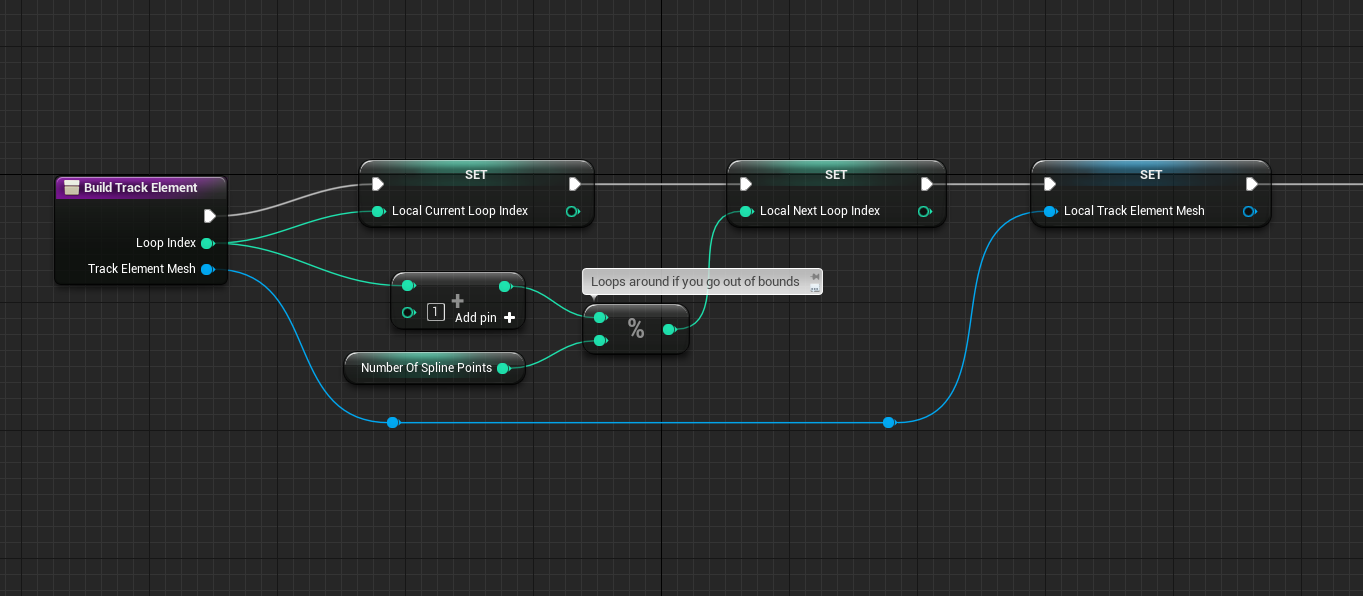
\includegraphics[width=.90\textwidth]{images/blueprint} @*)
\end{lstlisting}


Students have also suggested the minted package for pretty code listings.  We will consider this in future updates to the coding style at NTNU.




\input{inc/deployment}
\input{inc/testing}
\input{inc/discussion}
\input{inc/conclusion}


\bibliographystyle{ntnuthesis/ntnubachelorthesis}
\bibliography{inc/BachelorExample}

\appendix %after this line all chapters will have leters instead of numbers
%\chapter{Project Plan}
\label{app:plan}

This needs to be an example of including full PDF pages as an appendix

%\input{gantt}
\input{inc/meetinglog}
%\input{progressreviews}
%\input{worklog}

\end{document}
